\subsection{2-2 RunThreeToEight}

\subsubsection*{Code}

\inputgroovy[label=CreateSetsOfEight.groovy,firstline=4]{../ChapterExercises/src/c2/CreateSetsOfEight.groovy}
\inputgroovy[label=GenerateSetsOfThree.groovy,firstline=4]{../ChapterExercises/src/c2/GenerateSetsOfThree.groovy}
\inputgroovy[label=ListToStream.groovy,firstline=4]{../ChapterExercises/src/c2/ListToStream.groovy}
\inputgroovy[label=RunThreeToEight.groovy,firstline=5]{../ChapterExercises/src/c2/RunThreeToEight.groovy}

\subsubsection*{Questions}

\paragraph{ 1. What change is required to output objects containing six integers? }

To update the code to generate groups of 6 instead of 8 we can change the for loop in {\em CreateSetsOfEight.groovy} from \mintinline{groovy}{for ( int i in 0 .. 7 )} to \mintinline{groovy}{for ( int i in 0 .. 5 )}.

\subsubsection*{Results}

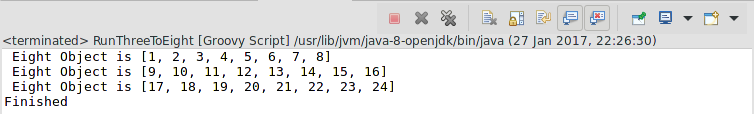
\includegraphics[width=\textwidth]{img/screenshots/2-2.png}
